% !TeX spellcheck = it_IT
\newpage
\section{Introduzione}
\begin{definition}[Base di dati]
	Insieme	\textbf{strutturato} e \textbf{organizzato} di dati omogenei utilizzati per il supporto allo svolgimento di attività (ente, azienda, ufficio, persona).
\end{definition}

\begin{definition}[Database Management System]
	Sistema software progettato per consentire la \textbf{creazione}, \textbf{manipolazione} e \textbf{interrogazione} di uno o più database in modo corretto ed efficiente.
\end{definition}

\noindent Le figure coinvolte nella costruzione di una \textit{base di dati} sono:
\begin{itemize}
	\item \textbf{Committente}
	\begin{itemize}
		\item Dirigente
		\item Operatore
	\end{itemize}
	\item \textbf{Fornitore}
	\begin{itemize}
		\item Direttore del progetto
		\item Analista
		\item Progettista di BD
		\item Programmatore di applicazioni che usano BD
	\end{itemize}
	\item \textbf{Manutenzione} e messa a punto
	\begin{itemize}
		\item Gestione del DBMS
		\item Amministratore del DBMS
	\end{itemize}
\end{itemize}
\subsection{Sistema informativo}
\begin{definition}[Sistema informativo]
	Una combinazione di \textbf{risorse},umane e materiali, e di procedure organizzate allo scopo di:
	\begin{itemize}
		\item \textbf{raccogliere}
		\item \textbf{archiviare}
		\item \textbf{elaborare} 
		\item \textbf{scambiare}
	\end{itemize}
	le \textbf{informazioni} necessarie alle \textbf{attività}:
	\begin{itemize}
		\item \textbf{operative} (servizio)
		\item di \textbf{programmazione} e \textbf{controllo} (gestione)
		\item di \textbf{pianificazione strategica} (governo)
	\end{itemize}
\end{definition}

\begin{center}
	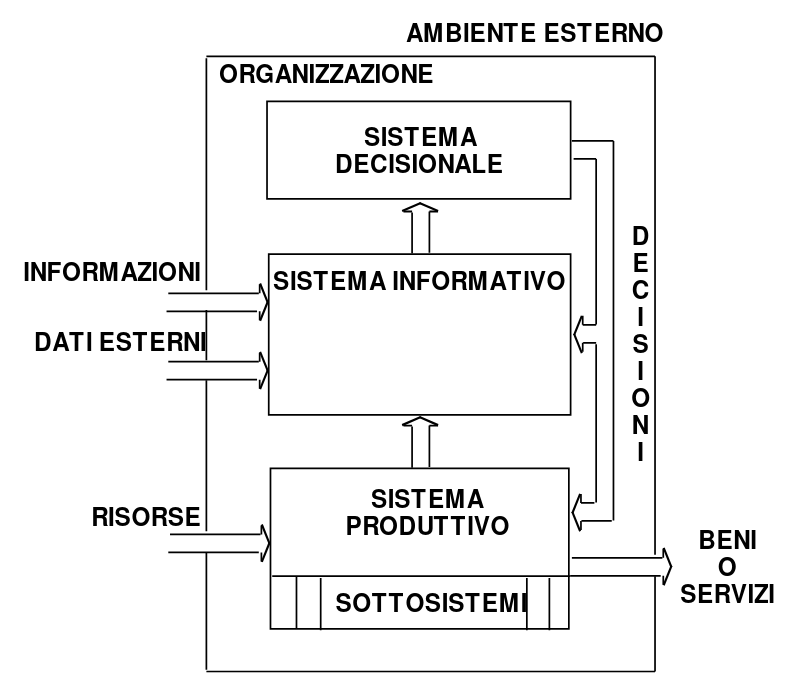
\includegraphics[scale=0.3]{sist_info.png}
\end{center}

\begin{example}[Azienda manifatturiera]
	Un'azienda manifatturiera avrà un sistema informativo che prevede la \textbf{gestione} di ordini (a clienti e fornitori), pagamenti e del magazzino, nonché la \textbf{pianificazione} e il controllo dei costi.
\end{example}

\subsection{Sistema informatico}
Nello specifico, si utilizza un \textbf{sistema informatico} per eseguire parte delle operazioni del sistema informativo in maniera \textbf{automatizzata}.
\begin{definition}[Sistema informatico]
	Insieme delle tecnologie informatiche e	della comunicazione (ICT) a supporto delle attività di
	un’organizzazione.
\end{definition}

\begin{center}
	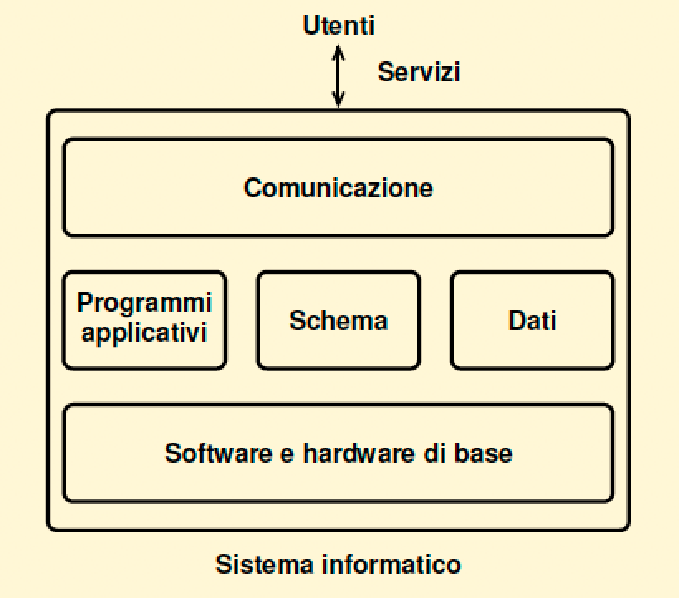
\includegraphics[scale=0.3]{sist_ict.png}
\end{center}
\subsubsection{Sistema informatico operativo}
In questo tipo di sistemi i dati sono organizzati in BD (gestite a loro volta da DBMS) e le applicazioni sono usate per svolgere attività \textbf{strutturate} e \textbf{ripetitive} (e.g. amministrazione, vendite, produzione, HR), ovvero \textbf{On-Line Transaction Processing} (operazioni \textbf{semplici} e con \textbf{pochi dati}).
\begin{definition}[Transaction Processing System]
	Sistema basato su transazioni: serie di azioni $S$ che se non andate a buon fine lasciano la BD nello stesso stato in cui era prima che $S$ iniziasse.
\end{definition}
\begin{center}
	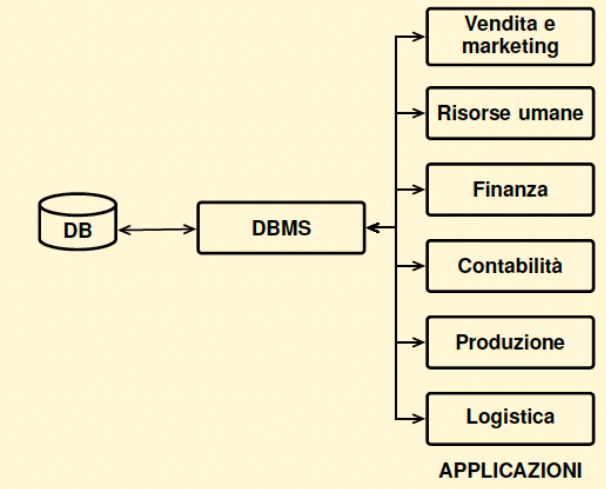
\includegraphics[scale=0.3]{sist_ict_op.png}
\end{center}

\subsubsection{Sistema informatico direzionale}
In questo tipo di sistemi i dati sono organizzati in una \textbf{Data Warehouse} e gestiti da un opportuno sistema. A differenza di quello operazionale, dove i dati sono aggiornati tempestivamente, in questo l'aggiornamento avviene in maniera periodica. Inoltre l'uso principale è per \textbf{On-Line Analytical Processing}, ovvero analisi dei dati a supporto delle decisioni (operazioni complesse e con molti dati).

\begin{definition}[Business Intelligence]
	Le applicazioni di Business intelligence sono strumenti di supporto ai processi di controllo delle prestazioni aziendali e di decisione manageriale.
\end{definition}

\begin{center}
	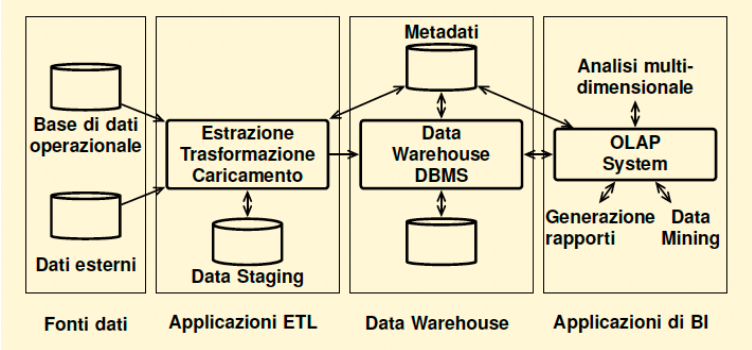
\includegraphics[scale=0.3]{sist_ict_dir.png}
\end{center}

Di seguito una tabella che riassume le differenze tra \textbf{OLTP} e \textbf{OLAP}:
\begin{center}
	\begin{tabular}{|c|c|c|}
		\hline
		& \textbf{OLTP} & \textbf{OLAP} \\
		\hline
		\textbf{Scopi} & Supporto operatività & Supporto decisioni \\
		\hline
		\textbf{Utenti} & Molti, esecutivi & Pochi, dirigenti e analisti \\
		\hline
		\textbf{Dati} & Pochi, analitici, relazionali & Molti, sintetici, multidimensionali \\
		\hline
		\textbf{Usi} & Noti a priori & Poco prevedibili \\
		\hline
		\textbf{Orientamento} & Applicazione & Soggetto \\
		\hline
		\textbf{Aggiornamento} & Frequente & Raro \\
		\hline
		\textbf{Visione dei dati} & Corrente & Storica \\
		\hline
		\textbf{Ottimizzati per} & Transazioni & Analisi \\
		\hline
	\end{tabular}
\end{center}

\subsubsection{Big Data}
Con questo termine ci si riferisce alle situazioni in cui DB o DW sono troppo lenti o restrittivi a causa della natura dei dati: \textbf{Volume}, \textbf{Varietà} e \textbf{Velocità}. In questo caso si usano approcci come:
\begin{itemize}
	\item NoSQL
	\item \textbf{Data mining}: fase di un processo interattivo e iterativo che cerca di estrarre modelli
	utili per prendere decisioni da un insieme di dati. Il modello sarà una rappresentazione concettuale che evidenzia alcune caratteristiche implicite
	\item Machine learning
	\item Data Lake
\end{itemize}

\subsection{Base di dati}

\begin{definition}[Base di dati]
	Una BD è una raccolta di \textbf{dati permanenti}, gestiti da un	elaboratore elettronico, suddivisi in:
	\begin{itemize}
		\item \textbf{Metadati} o schema: definizioni che \textbf{descrivono} i dati, pongono \textbf{restrizioni} su di essi, indicano le possibili \textbf{relazioni} ed \textbf{operazioni}
		\item \textbf{Dati}: rappresentazione di fatti conforme allo schema. Sono organizzati in insiemi \textbf{strutturati} ed \textbf{omogenei} fra i quali sono definite \textbf{relazioni}. Hanno le seguenti caratteristiche:
		\begin{itemize}
			\item \textbf{Molti} rispetto ai metadati
			\item \textbf{Permanenti} fino ad esplicita cancellazione
			\item Accessibili tramite \textbf{transazioni} (unità atomiche che non possono avere effetti parziali)
			\item \textbf{Protetti} da utenti ed errori
			\item Utilizzabili in \textbf{parallelo}
		\end{itemize}
	\end{itemize}
\end{definition}

\subsubsection{Sistemi per BD}
Il DBMS si occupa di garantire le caratteristiche della BD, controllandone i dati e gestendone l'accessibilità.

\begin{definition}[DBMS]
	Un \textbf{Database Management System} è un sistema centralizzato o	distribuito che offre opportuni linguaggi per:
	\begin{itemize}
		\item Definire lo \textbf{schema}
		\item Scegliere le \textbf{strutture dati} per \textit{memorizzazione} e \textit{accesso}
		\item \textbf{Memorizzare}, \textbf{recuperare} e \textbf{modificare} i dati interattivamente o da programmi
	\end{itemize}
\end{definition}

Il modello più diffuso è quello \textbf{relazionale} che utilizza come meccanismo principale di astrazione la \textbf{tabella}, ovvero un insieme di \textbf{record} con campi elementari (definiti assieme al nome dallo schema).\\
Le principali funzionalità del DBMS sono:
\begin{itemize}
	\item \textbf{Definizione} e \textbf{uso} della BD
	\item \textbf{Controllo} dei dati
	\item \textbf{Amministrazione}: definizione e modifica degli schemi, controllo e messa a punto del sistema, gestione dei diritti di accesso, strumenti di ripristino
	\item \textbf{Sviluppo}: strumenti per creare applicazioni. E.g. per produrre grafici, rapporti o GUI
\end{itemize}

\subsubsection{Linguaggi}
Per \textbf{definire} e \textbf{usare} una BD esistono due tipi di linguaggi:
\begin{itemize}
	\item \textbf{Data Definition Language}: per la definizione dello \textit{schema}
	\item \textbf{Data Manipulation Language}: permette agli operatori di accedere ai dati e modificarli
\end{itemize}
Dato che gli utenti sono di diversi tipi un DBMS deve prevedere più modalità d'uso: \textbf{GUI}, linguaggio di \textbf{querying} per non esperti, linguaggio di \textbf{programmazione} per integrarsi con applicazioni e linguaggio per lo \textbf{sviluppo di interfacce}.\\
Un esempio di linguaggio interattivo è \textbf{SQL} mentre un linguaggio ad-hoc è \textbf{PL/SQL}.

\paragraph{Livelli di descrizione} Ci sono tre livelli a cui descrivere i dati:
\begin{itemize}
	\item \textbf{Logico}: descrive la struttura degli insiemi di dati e delle relazioni fra loro, secondo un certo modello dei dati, senza nessun riferimento alla loro organizzazione fisica nella memoria permanente
	\item \textbf{Fisico}: descrive come vanno organizzati fisicamente i dati nelle memorie	permanenti e quali strutture dati ausiliarie prevedere per facilitarne l’uso
	\item \textbf{Esterno}: descrive come deve apparire la struttura della base di dati ad una certa applicazione
\end{itemize}
È necessario che ci sia \textbf{indipendenza} logica e fisica:
\begin{itemize}
	\item \textbf{Logica}: i programmi applicativi non devono essere modificati in seguito a modifiche dello schema logico
	\item \textbf{Fisica}: i programmi applicativi non devono essere modificati in seguito a modifiche dell’organizzazione fisica dei dati
\end{itemize}

\newpage
\subsubsection{Controllo di BD}
Una base di dati deve sempre garantire \textbf{integrità} (mantenimento delle proprietà specificate nello schema), \textbf{sicurezza} (chi e come può accedere ai dati) e \textbf{affidabilità}.

\paragraph{Affidabilità}
La BD deve garantire la protezione dei dati da malfunzionamenti HW, SW e da interferenze dovute ad accesso parallelo. 

\begin{definition}[Malfunzionamento]
	Evento a causa del quale la BD si può trovare in uno stato scorretto.
\end{definition}

Le transazioni permettono di garantire affidabilità.
\begin{definition}[Transazione]
	Una sequenza di azioni di lettura e scrittura in memoria permanente e di elaborazioni di dati in memoria temporanea, con	le seguenti proprietà:
	\begin{itemize}
		\item \textbf{Atomicità}: le transazioni che terminano prematuramente sono trattate dal sistema come se non fossero mai iniziate ed eventuali effetti sono annullati
		\item \textbf{Persistenza}: le modifiche di una transazione terminata normalmente non sono alterabili da eventuali	malfunzionamenti
		\item \textbf{Serializzabilità}: nel caso di transazioni concorrenti l’effetto è quello di una esecuzione seriale
	\end{itemize}
\end{definition}

In caso di malfunzionamento rilevato si procede con:
\begin{enumerate}
	\item Interruzione della transazione o del sistema
	\item Messa in atto di procedure di recupero
\end{enumerate}
I tipi di malfunzionamento sono:
\begin{center}
	\begin{tabular}{|c|c|}
		\hline
		\textbf{Tipo} & \textbf{Perdita dati} \\
		\hline
		Transaction & Nessuna \\
		\hline
		System & Memoria non permanente \\
		\hline
		Media & Memoria permanente \\
		\hline
	\end{tabular}
\end{center}

\subsubsection{Vantaggi e svantaggi}
I DBMS garantiscono:
\begin{itemize}
	\item \textbf{Indipendenza}, \textbf{integrità} e \textbf{sicurezza} dei dati
	\item Gestione degli accessi \textbf{concorrenti} e \textbf{interattiva} in maniera sicura
	\item \textbf{Amministrazione} dei dati
	\item Riduzione di \textbf{tempi} e \textbf{costi} di sviluppo
\end{itemize}
Al contrario però sono \textbf{complessi} e costosi da gestire perché rendono necessaria la definizione di uno \textbf{schema} e possono solo gestire dati \textbf{strutturati} ed \textbf{omogenei}.